\documentclass[oneside,final,12pt]{extreport}
\usepackage[utf8]{inputenc}
\usepackage[russian]{babel}
\usepackage{vmargin}
\setpapersize{A4}
\setmarginsrb{2.5cm}{2cm}{1.5cm}{2cm}{0pt}{0mm}{0pt}{13mm}
\usepackage{indentfirst}
\usepackage{amsmath,amsfonts}
\usepackage{enumerate}
\usepackage{amssymb}
\usepackage{graphicx}
\DeclareMathOperator*{\argmax}{\arg\!\max}
\sloppy
\begin{document}
 
\begin{titlepage}
\centerline{МОСКОВСКИЙ ГОСУДАРСТВЕННЫЙ УНИВЕРСИТЕТ ИМЕНИ М.В. ЛОМОНОСОВА}
\centerline{ФАКУЛЬТЕТ ВЫЧИСЛИТЕЛЬНОЙ МАТЕМАТИКИ И КИБЕРНЕТИКИ}
\centerline{КАФЕДРА ОПТИМАЛЬНОГО УПРАВЛЕНИЯ}
\centerline{\hfill\hrulefill\hrulefill\hfill}
\vfill
\vfill
\begin{Large}
\begin{centering}
Отчет по практикуму \\
Решение задач оптимизации \\
в системе Matlab \\
\end{centering}
\end{Large}
\vfill
\vfill
\begin{flushright}
Выполнил:\\
студент 413 группы\\
Ахрамеев П.К.\\
\vfill
Руководители практикума:\\
Артемьева Л.А.\\Будак Б.А.\\Ничипорчук А.В.\\
\end{flushright}
\vfill
\vfill
\centerline{Москва, 2013.}
\end{titlepage}
 
\setcounter{page}{2}
\tableofcontents
 
\chapter{Постановка задачи}
 
Рассмотрим задачу оптимального управления:
$$
\left\{\begin{aligned} & \dot x=f(x(t),u(t),t), \\ & x(t_0)=x_0, \\ & J(u)=\int_{t_0}^T f_0(x(t),u(t),t) \, dt+ \Phi(x(T))\rightarrow \min_{u \in U}. \end{aligned}\right.
$$
Здесь $x\in \mathbb{R}^n $ - вектор фазовых координат, $u$ - управление, $x_0$ - начальное состояние, $t\in[t_0,T]$; область управления
$$ U\subseteq L_2^r(t_0,T).$$
 
Требуется найти допустимое управление, которое обеспечивает минимизацию функционала $J(u)$.
 
Постановка задачи предполагает задание следующего набора исходных данных:
$$\left\{f(x,u,t),U,t_0,T,x_0,f_0(x,u,t),\Phi(x)\right\}.$$
 
\section{Задача с фиксированным правым концом}
 
Рассматривается задача оптимального управления:
$$ \left\{\begin{aligned} & \dot x=f(x(t),u(t),t), \\ & x(t_0)=x_0, x(T)=x_1, \\ & J(u)=\int_{t_0}^T f_0(x(t),u(t),t) \, dt+ \Phi(x(T))\rightarrow \min_{u \in U}. \end{aligned}\right. $$
 
Требуется найти допустимое управление, которое обеспечивает минимизацию функционала $J(u)$.
 
Постановка задачи предполагает задание следующего набора исходных данных:
$$\left\{f(x,u,t),U,t_0,T,x_0,x_1,f_0(x,u,t),\beta\right\}.$$
 
\chapter{Алгоритмы}
В данной главе описываются алгоритмы решения поставленной задачи следующими методами: методом проекции градиента и методом последовательных приближений. Для всех вышеперечисленных методов необходимо предварительное построение функции Гамильтона-Понтрягина
$$H(x,t,u,\psi)=-f_0(x,t,u)+\langle f(x,t,u),\psi(t)\rangle.$$
Алгоритмы решения задачи с фиксированным правым концом сводятся к алгоритмам решения основной задачи.
 
\section{Метод проекции градиента} 
Общая схема метода:\\
Пусть $u_0$ - некоторое начальное приближение. Далее будем строить последовательность ${u_k}$ по правилу:
$$ u_{k+1}=Pr_U(u_k-\alpha_kJ'(u_k)), k=0,1,\dots$$
где $\alpha_k$ - положительная величина.\\
Если на некоторой итерации оказалось, что $u_{k+1}=u_k$, то процесс прекращают. В этом случае точка $u_k$ удовлетворяет необходимому условию оптимальности.\\
Известно, что если функции $f^0$, $f$, $\Phi$ непрерывны по совокупности своих аргументов вместе со своими частными производными по переменным $x$, и при $(x,u,t)\in E^n E^r[t_0, T]$ и, кроме того, функции вместе со своими производными по переменным $x$ и $u$ являются Липшицевыми с некоторой 
константой $L \geqslant 0$, 
тогда функция $J(u)$ непрерывна и 
дифференцируема по $u=u(t)$ в норме $L^{r}_2(0, T)$ всюду на $L^{r}_2(0, T)$, 
причем ее градиент $J'(u)=J'(u,t) \in L^{r}_2(0, T)$ в точке $u=u(t)$ представим в виде
$$J'(u)=-H_u(x(t,u),t,u(t),\psi(t,u))|_{x=x(t,u),u=u(t),\psi=\psi(t,u)}=$$ 
$$f^0_u(x(t,u),u(t),t)-(f_u(x(t,u),u(t),t))^T\psi(t,u), \ t_0 \leqslant t \leqslant T.$$

\noindent Также необходимо вычислить функцию Гамильтона-Понтрягина:
$$H(x,t,u,\psi)=-f_0(x,u,t)+\langle f(x,u,t),\psi(t)\rangle_{R^{n}}, \ (\psi)^T=(\psi_1, \psi_2,...,\psi_n).$$
\newpage
\textbf{Минимизация функционала методом проекции градиента.}
\begin{equation}
\left \{\begin{aligned}
& \dot{x} = f(x,u,t)\\
& x(t_0)=x_0, \ t_0 \leqslant t \leqslant T\\
\end{aligned} \right. 
\end{equation}
Будем называть систему (1) основной системой.

\begin{equation}
\left \{
\begin{aligned}
& \dot{\psi} = -H_x(x,t,u,\psi),\ t_0 \leqslant t \leqslant T \\
& \psi(T) = -\Phi_x(x(T))
\end{aligned} \right.
\end{equation}

Будем называть систему (2) сопряженной системой.

В качестве начального приближения выберем $u_0(t) \in U$

Алгоритм для 1 итерации:
\begin{enumerate}
\item Управление $u_k(t)$ подставляем в основную систему (1), решаем ее, находим $x_k(t)$.
\item Подставляем $u_k(t)$ и $x_k(t)$ в сопряженную систему (2), решаем ее, находим $\psi_k(t)$.
\item Управление на каждом шаге рассчитывается по формуле $u_{k+1}=pr_U(u_k-\alpha_kJ'(u_k))$, \ $\alpha_k \geqslant 0$ - шаг метода.\\ Градиент функционала $J'(u)=-H_u(x(t,u),t,u(t),\psi(t,u))$

\end{enumerate}
Критерии останова
\begin{itemize}
\item По количеству итераций
\item По управлению
$$\left \|u_k(t)-u_{k+1}(t)\right \| < \epsilon$$
\item По функционалу
$$\left |J(u_k(t))-J(u_{k+1}(t))\right | < \epsilon$$
\end{itemize}

\section{Пример работы метода проекции градиента}
 
В качестве примера я привожу решение задачи простого движения.

$$
\begin{cases}
\dot{x_1}=u_1(t), \ 0 \leqslant t \leqslant 2\\ 
x_1(0)=1,\\
J(u)=\int_0^2 x_1^2(t) \, dt\rightarrow inf,\\
\|u_1(t)\|\leqslant1.
\end{cases}
$$

На рисунке ~\ref {simpleMpgPic} можно увидеть, как эти параметры корректно ввести в программу. Для удобства пользователя этот пример можно быстро выбрать в списке примеров (через выпадающий список в верхнел левом углу экрана или через меню Файл-Открыть).

\begin{figure}[!h]
\centering
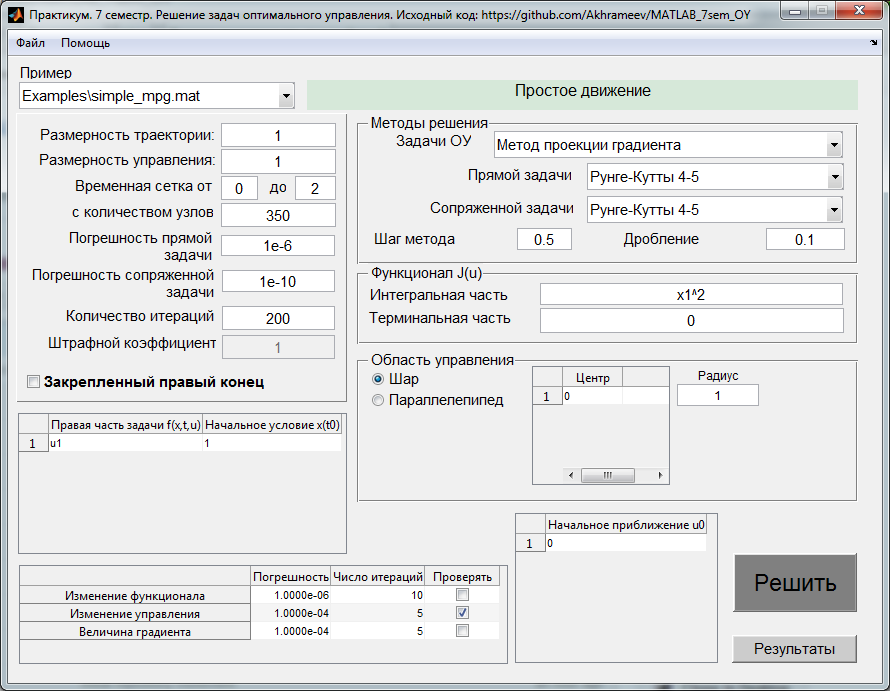
\includegraphics[scale=0.7]{simple_mpg.png}
\caption{Экран с параметрами для расчета задачи простого движения методом проектции градиента}
\label{simpleMpgPic}
\end{figure}

После появления кнопки "Результат" и клика по ней возникнет окно, изображенное на рисунке ~\ref {simpleMpgResPic}.
 
\begin{figure}[!h]
\centering
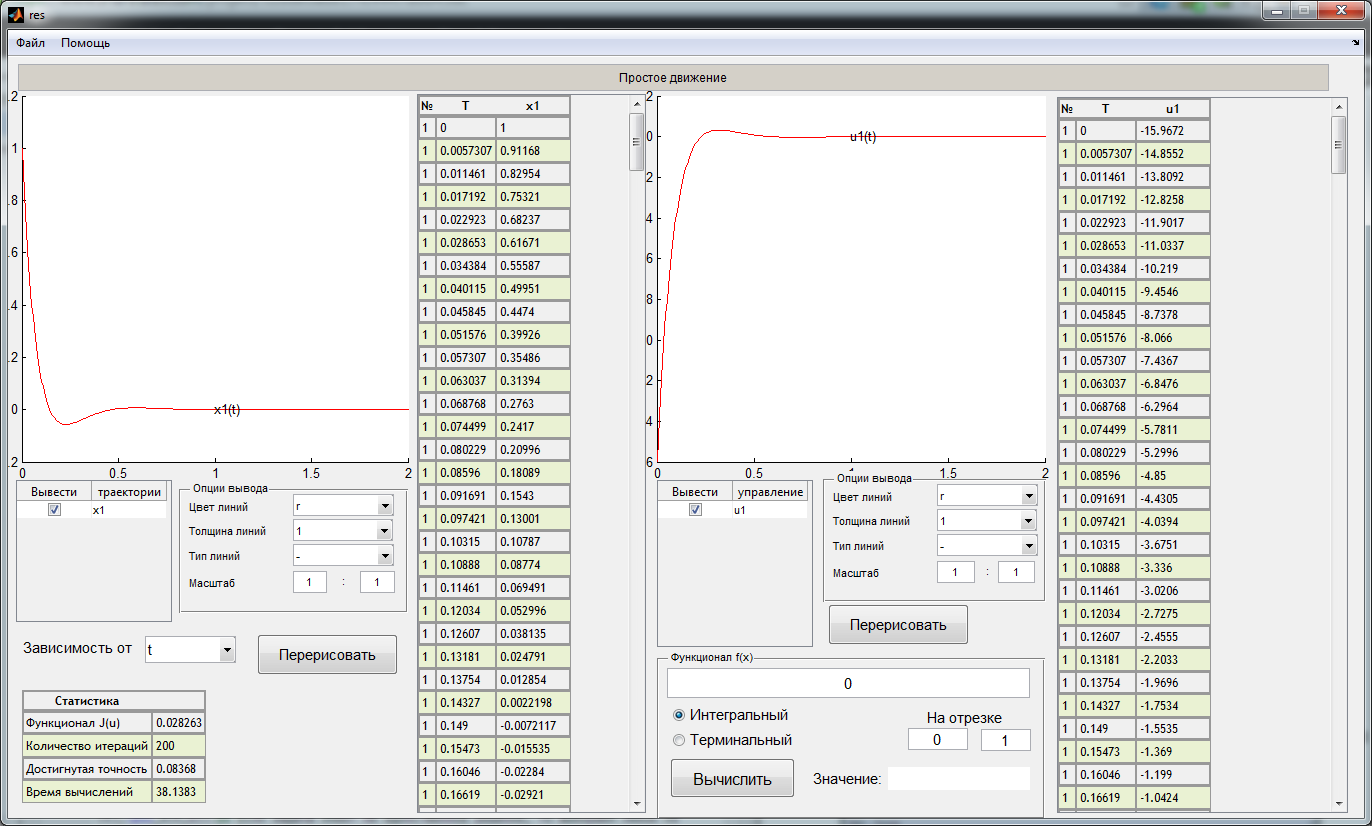
\includegraphics[scale=0.45]{simple_mpg_res.png}
\caption{Экран с результатами расчета задачи простого движения методом проектции градиента}
\label{simpleMpgResPic}
\end{figure}

\section{Метод последовательных приближений} 
Отличие от метода проекции градиента в том, что на каждом шаге необходимо решать задачу максимизации
$$H_u(x_k(t,u),t,u_{k+1}(t),\psi_k(t,u))= arg \max \limits_{u \in U} H_u(x_k(t,u),t,u_k(t),\psi_k(t,u)).$$ Если задача имеет не единственное решение, то выбираем любое из возможных значений. После этого переходим к следующей итерации. 
Если процесс последовательных приближений сходится, то продолжаем его до тех пор, пока последующие приближения не будут отличаться друг от друга в пределах заданной точности.
\textbf{Минимизация функционала методом проекции градиента.}
\begin{equation}
\left \{\begin{aligned}
& \dot{x} = f(x,u,t)\\
& x(t_0)=x_0, \ t_0 \leqslant t \leqslant T
\end{aligned} \right. 
\end{equation}
Будем называть систему (3) основной системой.

\begin{equation}
\left \{
\begin{aligned}
& \dot{\psi} = -H_x(x,t,u,\psi),\ t_0 \leqslant t \leqslant T \\
& \psi(T) = -\Phi_x(x(T))
\end{aligned} \right.
\end{equation}
Будем называть систему (4) сопряженной системой.

В качестве начального приближения выберем $u_0(t) \in U$.

Алгоритм для 1 итерации:
\begin{enumerate}
\item Управление $u_k(t)$ подставляем в основную систему (1), решаем ее, находим $x_k(t)$.
\item Подставляем $u_k(t)$ и $x_k(t)$ в сопряженную систему (2), решаем ее, находим $\psi_k(t)$.
\item Находим очередное приближение оптимального управления $$u_{k+1}(t)= arg \max \limits_{u \in U} H(x_k(t),t,u(t),\psi_k(t)),$$ решая задачу максимизации.
\item Проверяем монотонность: если $J(u_{k+1})<J(u_k),$ то дробим шаг.
\item Если больше k дроблений без эффекта, то останавливаемся.
\end{enumerate}

\noindent \textbf{Улучшения метода последовательных приближений}

\noindent \textbf{Коррекция №1}

Рассматривается семейство задач
\begin{equation}
\left \{
\begin{aligned}
& \dot{x} = \epsilon f(x,u,t)\\
& x(t_0)=x_0
\end{aligned} \right.
\end{equation}
или
\begin{equation}
\left \{
\begin{aligned}
& \dot{x} = f(x,u,t)\\
& x(t_0)=x_0, 
\end{aligned} \right.
\end{equation}
где $0< \epsilon <1$.

Вводим сетку $0< \epsilon_1 < \epsilon_2 < \epsilon_3 <...<\epsilon_l=1$. l - параметр
Схема коррекции:
\begin{enumerate}
\item Запускаем базовую схему для задачи (6) с $\epsilon_0$ и начальным приближением $u_0(t)$. Ее решением будет какое-то управление $\bar{u}(t)$, причем $J(\bar{u}) \leqslant J(u_0)$.
\item Найденное на шаге 1 $\bar{u}(t)$ полагаем следующей итерацией $u_1(t)$, запускаем базовую схему из $u_1(t)$ для задачи (6) с $\epsilon_1$. И так далее.
\item На шаге l мы уже запустим фактически базовую схему для исходной задачи (т.к. $\epsilon_1=1$), но из более хорошего начального приближения.
\end{enumerate}

\noindent \textbf{Коррекция №2}
Начальное приближение $u_0(t)$~--- базовая схема закончила работу на $\breve u_0(t)$. В качестве $u_1(t)$ берем некую комбинацию $u_0(t)$ и $\breve u_0(t).$

I.
$u_1(t)=\alpha u_0(t)+(1-\alpha)\breve u_0(t)$, причем $\alpha=arg \min \limits_{\beta \in [0,1]} J(\beta u_0(t)+(1-\beta)\breve u_0(t))$. На практике просто перебираем конечное число $\alpha:$\\ $0=\alpha_0<\alpha_1<\alpha_2<...<\alpha_{\rho}=1$.

II.
$$
 u_1(t)=
\left \{\begin{aligned}
& u_0(t), \  t \in[\theta]\\
& \breve u_0(t), \  t \in(t_0, T)/\theta \\
\end{aligned} \right.
$$
 
\section{Пример работы метода последовательных приближений}
 
В качестве примера я привожу решение задачи минимального движения.

$$
\begin{cases}
\dot{x_1}=u_1(t), \ 0 \leqslant t \leqslant 2\\ 
x_1(0)=1,\\
J(u)=\int_0^2 x_1^2(t) + u_1^2(t) \, dt\rightarrow inf,\\
\|u_1(t)\|\leqslant1.
\end{cases}
$$

На рисунке ~\ref {minimalMppPic} можно увидеть, как эти параметры корректно ввести в программу. Для удобства пользователя этот пример можно быстро выбрать в списке примеров (через выпадающий список в верхнел левом углу экрана или через меню Файл-Открыть).

\begin{figure}[!h]
\centering
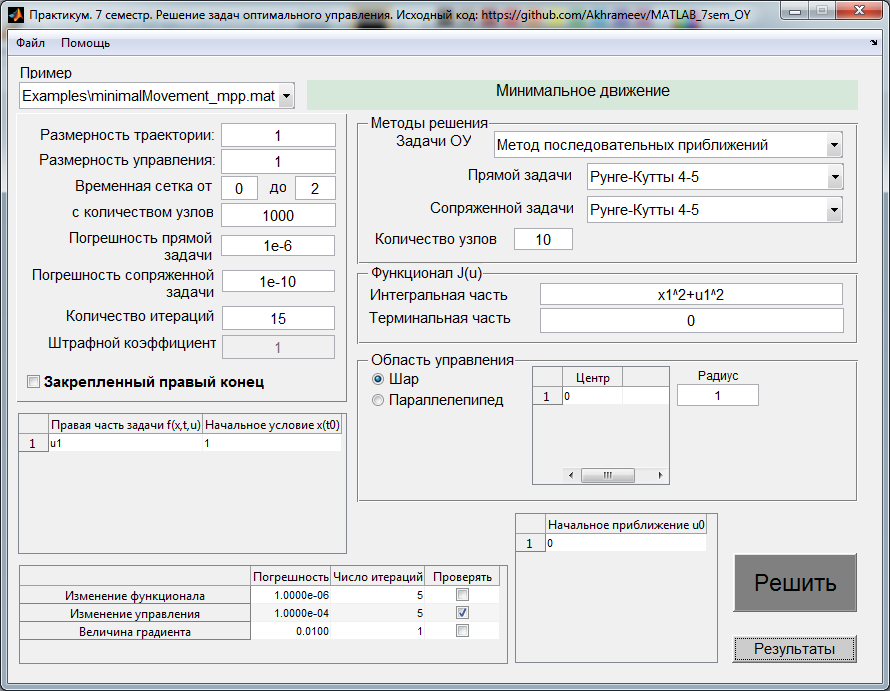
\includegraphics[scale=0.7]{minimalMovement_mpp.png}
\caption{Экран с параметрами для расчета задачи минимального движения методом последовательного приближения}
\label{minimalMppPic}
\end{figure}

После появления кнопки "Результат" и клика по ней возникнет окно, изображенное на рисунке ~\ref {minimalMppResPic}.
 
\begin{figure}[!h]
\centering
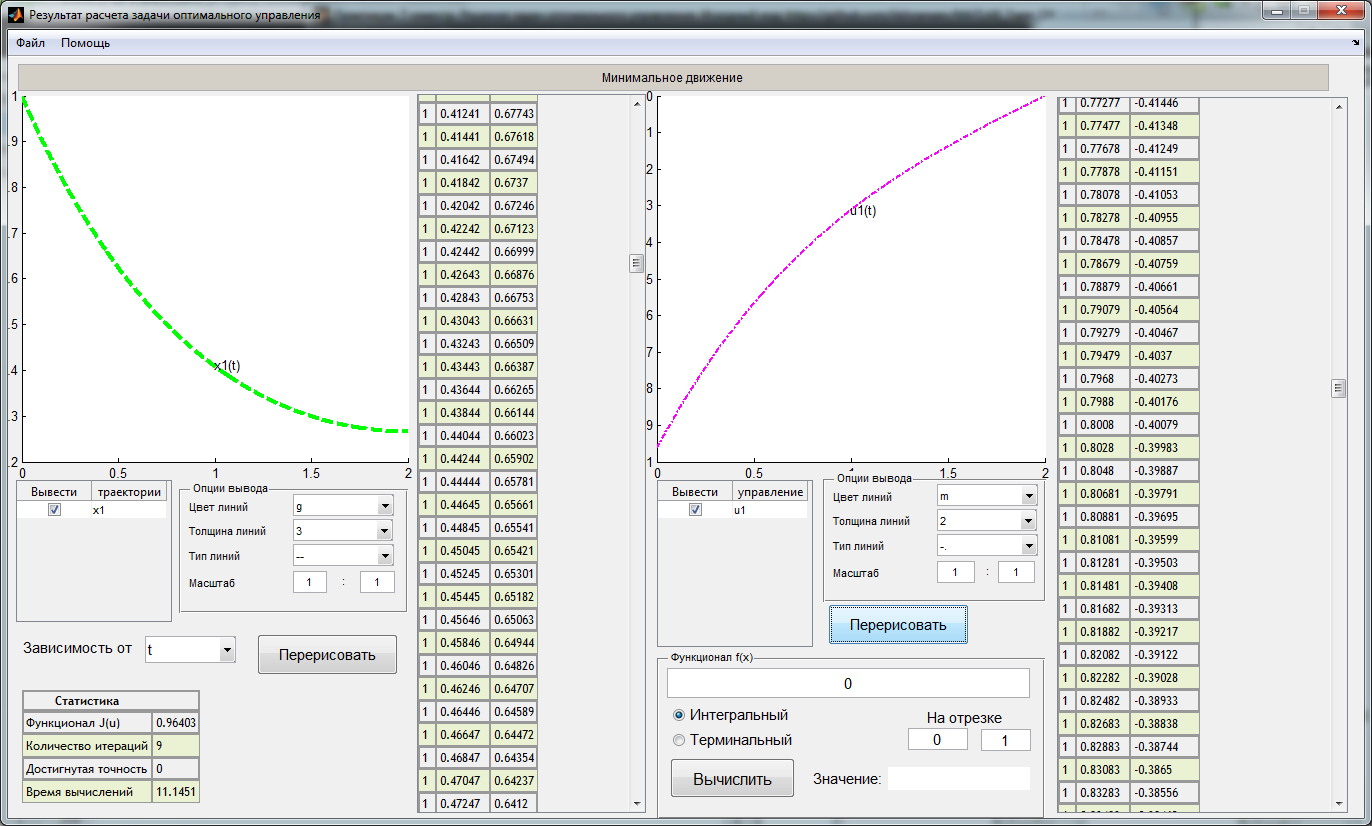
\includegraphics[scale=0.45]{minimalMovement_mpp_res.png}
\caption{Экран с результатами расчета задачи минимального движения методом последовательного приближения}
\label{minimalMppResPic}
\end{figure}
 
\chapter{Программная реализация}
 
В среде matlab была написана программа, реализующая метод проекции градиента и метод
последовательных приближений для задач оптимального управления.

\section{Руководство по работе с программой}

Чтобы решить конкретную задачу надо:

\begin{enumerate}
\item Задать задачу оптимального управления. Это можно сделать через меню Файл-Открыть, через выпадающий список в правом верхнем углу или ввести параметры вручную.
\item Задать геометрические ограничения на управления
Управления можно рассматривать на шаре или на параллелепипеде.
\item Выбрать метод и задать параметры для него.
\item Нажать на кнопку "Решить"
По окончанию расчета появится кнопка "Результат". При клике на неё откроется новое окно с временем работы программы, значением функционала, а также графиками управления и траектории. Также будет доступна информация о значениях управления и траектории на разбиении по времени t.

\end{enumerate}
 
\begin{thebibliography}{0}
\bibitem{bey:meth} И.~В.~Бейко, Б.~Н.~Бублик, П.~Н.~Зинько.
\emph{Методы и алгоритмы решения задач оптимизации}.
Вища школа, 1983.
\bibitem{rov:opt} E.~A.~Rovenskaya, D.~V.~Kamzolkin.
\emph{Infinite Horizon Optimal Control with Applications in Growth Theory: Practical Guide}.
MSU CMC Publication Department, MAKS Press, Moscow, Russia, 2009.
\end{thebibliography}
 
\end{document}
